\chapter{Analisis}
\label{chap:analisis}

\section{Analisis Sistem Kini}
\label{sec:analisiskini}
Pada halaman utama KIRI (dapat dilihat pada gambar \ref{fig:3_KIRI_main}), terdapat beberapa bagian yaitu:

\begin{enumerate}
    		\item \textbf{Peta}
    		\item \textbf{Form Samping} yang terdiri dari beberapa bagian, yaitu:
    		\begin{enumerate}
    			\item \textbf{Dropdown Menu Kota}, untuk memilih kota tujuan.
    			\item \textbf{Dropdown Menu Bahasa}, untuk memilih bahasa yang akan ditampilkan pada aplikasi.
    			\item \textbf{Textfield ``From'' \& ``To''}, untuk menerima masukan pengguna.
    			\item \textbf{Tombol Swap}, untuk menukar isi masukan pengguna antara Textfield ``From'' dan Textfield ``To''.
    			\item \textbf{Tombol Reset}, untuk menyetel ulang peta dan masukan pengguna.
    			\item \textbf{Tombol Find}, untuk mencari pencarian rute.
    		\end{enumerate}
\end{enumerate}

\begin{figure}[H]
	\centering
	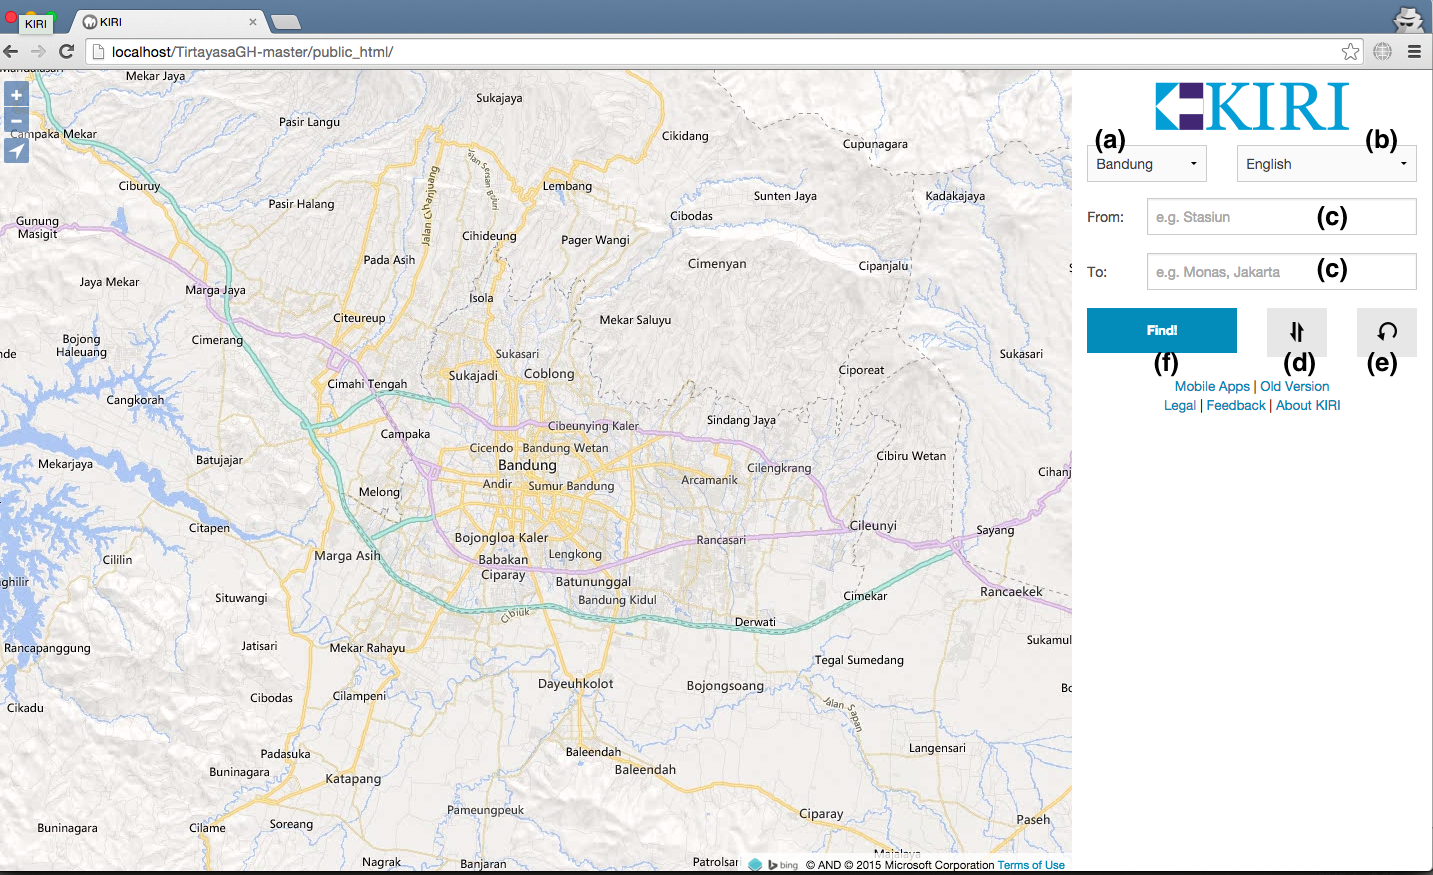
\includegraphics[scale=0.3]{Gambar/KIRI-main}
	\caption{Halaman Utama KIRI} 
	\label{fig:3_KIRI_main}
\end{figure}

\subsection{Peta}
Peta pada aplikasi KIRI berfungsi untuk menerima masukan pengguna berupa klik,  menampilkan lokasi start dan finish, serta menampilkan hasil pencarian rute.

\begin{figure}[H]
	\centering
	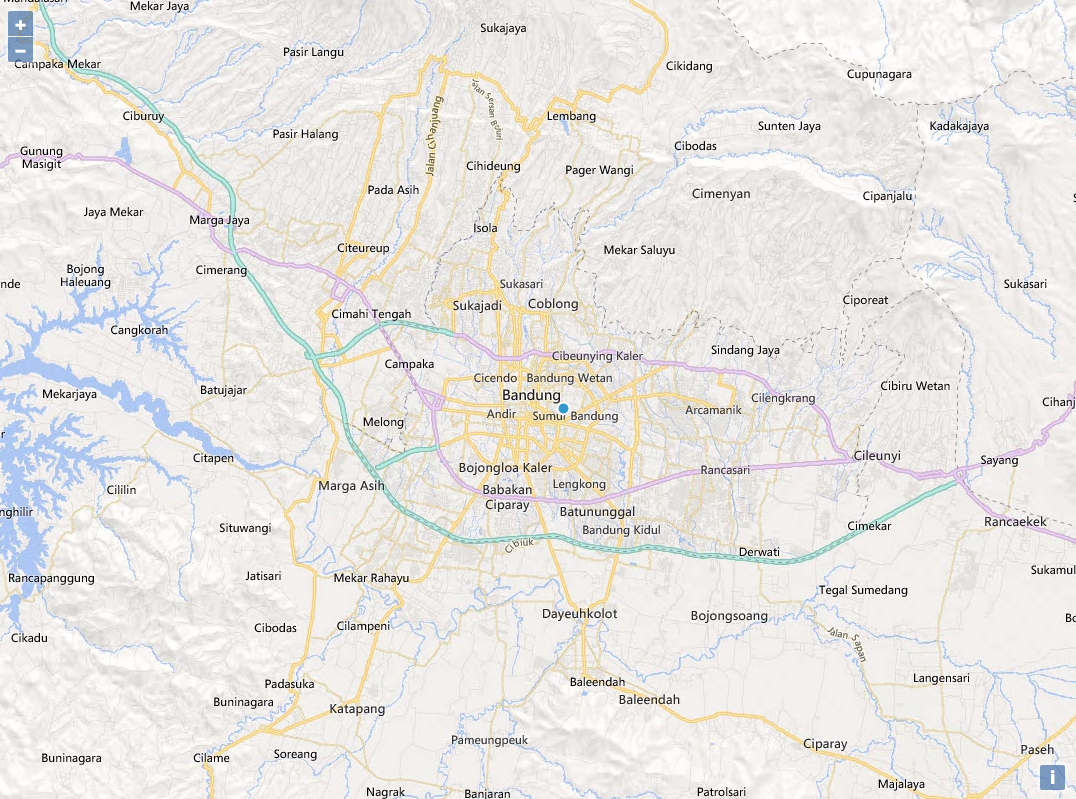
\includegraphics[scale=0.4]{Gambar/KIRI-peta}
	\caption{Peta pada KIRI} 
	\label{fig:3_KIRI_peta}
\end{figure}

KIRI menggunakan OpenLayers yang berbasis JavaScript untuk memuat peta pada halaman web. Pertama melakukan deklarasi peta yang digunakan menggunakan BingMaps. Penggunaan BingMaps membutuhkan dua parameter, yaitu \textit{key} yang merupakan kunci untuk menggunakan BingMaps dan \textit{imagerySet} yang merupakan tipe peta pada BingMaps. Contoh deklarasi peta dapat dilihat pada kode listing \ref{lst_3_php_peta_bing}.

\begin{lstlisting}[caption=Deklarasi peta BingMaps,label = {lst_3_php_peta_bing}]
var mapLayer = new ol.layer.Tile(
{
	source : new ol.source.BingMaps(
		{
			key : 'AuV7xXD6_UMiQ5BLoZr0xkpjLpzWqMT55772Q8XtLIQeuDebHPKiNXSlZXxEr1GA',
			imagerySet : 'Road'
		})
});
var resultVectorSource = new ol.source.Vector();
var inputVectorSource = new ol.source.Vector();
\end{lstlisting}

Untuk menambahkan fitur pada peta OpenLayers, seperti membuat \textit{marker} pada peta dan membuat rute pada peta dapat dicapai dengan menyiapkan objek \verb!ol.source.Vector!.

Setelah deklarasi peta beserta menyiapkan fitur yang terdapat pada peta, memasukkan semua fitur pada \textit{layers} dan \textit{target} untuk memasukkan \textit{id tag} yang digunakan pada HTML seperti pada kode listing \ref{lst_3_php_peta_instansiasi}.

\begin{lstlisting}[caption=Menentukan target tampilan peta,label = {lst_3_php_peta_instansiasi}]
var map = new ol.Map(
	{
		...
		layers : [ mapLayer, new ol.layer.Vector({source: inputVectorSource}), new ol.layer.Vector({source: resultVectorSource}) ],
		target : 'map'
});
\end{lstlisting}

\subsection{Form Samping}
Form yang terdapat pada halaman utama KIRI (Gambar \ref{fig:3_KIRI_form}) terdiri dari:
\begin{figure}[H]
	\centering
	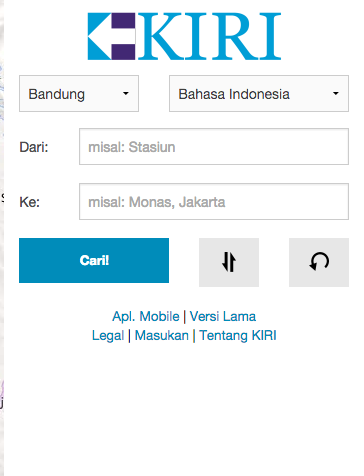
\includegraphics[scale=0.5]{Gambar/KIRI-form}
	\caption{Form pada KIRI} 
	\label{fig:3_KIRI_form}
\end{figure}

\subsubsection{Dropdown Menu Kota}
\textit{Dropdown} yang berfungsi untuk memilih kota tujuan (Gambar \ref{fig:3_KIRI_drop_kota}).

\begin{figure}[H]
	\centering
	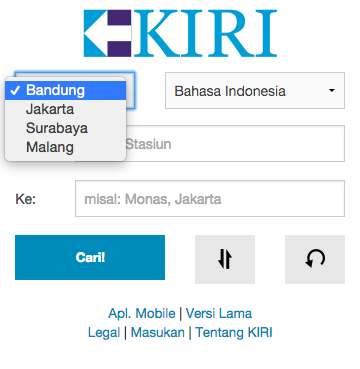
\includegraphics[scale=0.5]{Gambar/KIRI-drop-kota}
	\caption{Dropdown Menu Kota pada KIRI} 
	\label{fig:3_KIRI_drop_kota}
\end{figure}

Melakukan deklarasi variabel \verb!regioninfos! sebagai \textit{associated array} pada file \textit{constants.php}. Setiap kota direpresentasikan sebagai \verb!variabel proto_region_KOTA! dimana KOTA adalah kota yang ada pada KIRI. Setiap \verb!variabel proto_region_KOTA! merupakan \textit{array} dengan indeks:
\begin{enumerate}
	\item \textit{lat} sebagai garis lintang,
	\item \textit{lon} sebagai garis bujur,
	\item \textit{zoom} sebagai tingkat \textit{zoom} untuk memperbarui peta,
	\item \textit{name} untuk menampilkan nama kota,
	\item \textit{searchplace\_regex} untuk pencarian rute pada pilihan kota.
\end{enumerate} 
Kode dapat dilihat pada kode listing \ref{lst_3_php_dropdown_kota_regioninfos}.

\begin{lstlisting}[caption=Deklarasi variabel regioninfos,label = {lst_3_php_dropdown_kota_regioninfos}]
..
/** Different parameters for different regions. */
	$regioninfos = array(
		$proto_region_bandung => array(
			'lat' => -6.91474,
			'lon' => 107.60981,
			'radius' => 17000,
			'zoom' => 12,
			'searchplace_regex' => ', *(bandung|bdg)$',
			'name' => 'Bandung'
		),
		$proto_region_jakarta => array(
			'lat' => -6.21154,
			'lon' => 106.84517,
			'radius' => 15000,
			'zoom' => 11,
			'searchplace_regex' => ', *(jakarta|jkt)$',
			'name' => 'Jakarta'
		),
		$proto_region_surabaya => array(
			'lat' => -7.27421,
			'lon' => 112.71908,
			'radius' => 15000,
			'zoom' => 12,
			'searchplace_regex' => ', *(surabaya|sby)$',
			'name' => 'Surabaya'
		),
		$proto_region_malang => array(
			'lat' => -7.9812985,
			'lon' => 112.6319264,
			'radius' => 15000,
			'zoom' => 13,
			'searchplace_regex' => ', *(malang|mlg)$',
			'name' => 'Malang'				
		)
	);
..
\end{lstlisting}

Untuk menampilkan pilihan kota, pertama mengambil \textit{array} \verb!regioninfos!, lalu melakukan pengulangan sebanyak nilai yang terdapat pada \verb!regioninfos!. Dalam pengulangan tersebut, menulis \textit{tag} HTML \verb!option! sesuai dengan \textit{name} yang terdapat pada \verb!regioninfos!, jika \verb!regioninfos! dengan indeks\verb!`name'! sama dengan \textit{region} pengguna, maka opsi tersebut akan terpilih. Kode dapat dilihat pada kode listing \ref{lst_3_php_dropdown_kota_tampilan}

\begin{lstlisting}[caption=Menampilkan pilihan kota kepada pengguna ,label = {lst_3_php_dropdown_kota_tampilan}]
..
<select class="fullwidth" id="regionselect">
	<?php
		foreach ($regioninfos as $key => $value) {
			print "<option value=\"$key\"";
			if ($key == $region) {
				print " selected";
			}
			print ">" . $value['name'] . "</option>\n";
		}
	?>
</select>
..
\end{lstlisting}

Untuk memperbarui peta, KIRI menggunakan fungsi JavaScript dengan menerima dua parameter, yaitu \verb!newRegion! dan \verb!updateCookie!. Pertama membuat \textit{cookie} dengan kunci \verb!region!, lalu membuat variabel \verb!point! dengan mengubah String menjadi format garis lintang dan garis bujur dari titik tengah peta yang dituju. Untuk memperbarui peta dengan mengatur titik tengah pada peta yaitu memanggil \textit{method} \verb!setCenter! yang menerima parameter \verb!ol.proj.transform! yang berisi garis lintang dan bujur. Setelah itu, mengatur tingkat \textit{zoom} dengan memanggil \textit{method} \verb!setZoom! dengan parameter berupa tingkat \textit{zoom} dari peta yang dituju. Kode dapat dilihat pada kode listing \ref{lst_3_php_dropdown_kota_update}

\begin{lstlisting}[caption=Fungsi JavaScript untuk memperbarui peta ,label = {lst_3_php_dropdown_kota_update}]
/**
 * Updates the region information in this page.
 */
function updateRegion(newRegion, updateCookie) {
	region = newRegion;
	setCookie('region', region);
	var point = stringToLonLat(regions[region].center);
	map.getView().setCenter(ol.proj.transform(point, 'EPSG:4326', 'EPSG:3857'));
	map.getView().setZoom(regions[region].zoom);
}
\end{lstlisting}

Untuk mengubah tipe data String menjadi \textit{array} Float yang berguna menjadi garis lintang dan garis bujur dengan cara memanggil \textit{method} \textbf{split} dengan parameter `,' yang berfungsi membuang `,' dan menjadikan \textit{array}. Setelah menjadi \textit{array}, String tersebut masing-masing dijadikan ke tipe data Float dengan cara memanggil \textit{method} \textbf{parseFloat} dengan parameter String yang ingin dijadikan Float. Kode dapat dilihat pada kode listing \ref{lst_3_php_dropdown_kota_parse}.

\begin{lstlisting}[caption=Fungsi JavaScript untuk mengubah String menjadi \textit{array} Float ,label = {lst_3_php_dropdown_kota_parse}]
/**
 * Converts "lat,lng" into lonlat array
 * @return the converted lonlat array
 */
function stringToLonLat(text) {
	var latlon = text.split(/,\s*/);
	return [parseFloat(latlon[1]), parseFloat(latlon[0])];
}
\end{lstlisting}

\subsubsection{Dropdown Menu Bahasa}
\textit{Dropdown} yang berfungsi untuk memilih bahasa yang akan ditampilkan pada aplikasi (Gambar \ref{fig:3_KIRI_drop_bahasa}).

\begin{figure}[H]
	\centering
	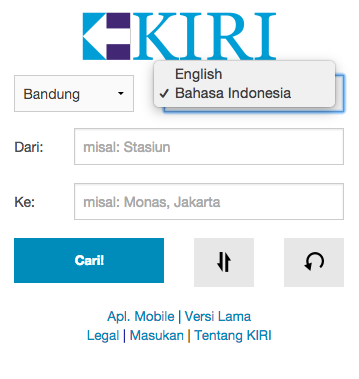
\includegraphics[scale=0.5]{Gambar/KIRI-drop-bahasa}
	\caption{Dropdown Menu Bahasa pada KIRI} 
	\label{fig:3_KIRI_drop_bahasa}
\end{figure}

Untuk menampilkan pilihan bahasa, menggunakan \textit{tag} HTML \verb!option!. Pada bagian ini, hanya cek jika sudah dilakukan lokalisasi ke Bahasa Indonesia, maka opsi yang terpilih adalah Bahasa Indonesia. Kode dapat dilihat pada \ref{lst_3_php_dropdown_bahasa_tampilan}

\begin{lstlisting}[caption=Menampilkan pilihan bahasa kepada pengguna ,label = {lst_3_php_dropdown_bahasa_tampilan}]
..
<select class="fullwidth" id="localeselect">
	<option value="en">English</option>
	<option value="id"
		<?php if ($locale == $proto_locale_indonesia) print " selected"; ?>>Bahasa
		Indonesia</option>
</select>
..
\end{lstlisting}

Ketika memilih \textit{dropdown} bahasa, memanggil \textit{method} JavaScript dengan parameter berupa fungsi yang berisi menambahkan \textit{query parameter} \verb!locale!. Kode dapat dilihat pada kode listing \ref{lst_3_php_dropdown_bahasa_fungsi}.

\begin{lstlisting}[caption=Fungsi JavaScript untuk Internationalization ,label = {lst_3_php_dropdown_bahasa_fungsi}]
..
// Event handlers
var localeSelect = $('#localeselect');
localeSelect.change(function() {
	// IE fix: when window.location.origin is not available 
	if (!window.location.origin) {
		window.location.origin = window.location.protocol + "//" + window.location.hostname + (window.location.port ? ':' + window.location.port: '');
	}
	window.location.replace(window.location.origin + "?locale=" + localeSelect.val());
});
..
\end{lstlisting}


\subsubsection{Textfield}
\textit{Textfield} pada KIRI menggunakan PHP agar dapat dilakukan proses Internationalization, seperti pada kode listing \ref{lst_3_php_textfield_from} untuk \textit{textfield} tempat asal dan kode listing \ref{lst_3_php_textfield_to} untuk \textit{textfield} tempat tujuan. Textfield pada KIRI dapat menerima dua masukan pengguna, yaitu:

\begin{lstlisting}[caption=Menampilkan \textit{textfield} tempat awal kepada pengguna ,label = {lst_3_php_textfield_from}]
..
<div class="small-2 columns">
	<label for="startInput" class="inline"><?php print $index_from; ?></label>
</div>
<div class="small-10 columns">
	<input type="text" id="startInput" value=""
		placeholder="<?php print $index_placeholder_start; ?>">
</div>
..
\end{lstlisting}

\begin{lstlisting}[caption=Menampilkan \textit{textfield} tempat tujuan kepada pengguna ,label = {lst_3_php_textfield_to}]
..
<div class="small-2 columns">
	<label for="finishInput" class="inline"><?php print $index_to; ?></label>
</div>
<div class="small-10 columns">
	<input type="text" id="finishInput" value=""
		placeholder="<?php print $index_placeholder_finish; ?>">
</div>
..
\end{lstlisting}

\begin{enumerate}
	\item \textbf{Textfield dengan Masukan Nama Tempat}, pengguna dapat memasukkan nama tempat asal dan tujuan dan KIRI akan menampilkan sugesti nama tempat (Gambar \ref{fig:3_KIRI_textfield_nama})
	
	\begin{figure}[H]
		\centering
		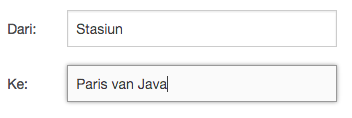
\includegraphics[scale=0.5]{Gambar/KIRI-textfield-nama}
		\caption{Input User(Nama Tempat)} 
		\label{fig:3_KIRI_textfield_nama}
	\end{figure}
	
	\item \textbf{Textfield dengan Masukan Klik Peta}, pengguna melakukan klik pada peta. Dengan melakukan klik pada peta, textfield tempat asal dan tujuan akan akan secara otomatis terisi oleh koordinat masing-masing tempat (Gambar \ref{fig:3_KIRI_textfield_koord}).
	
\begin{figure}[H]
	\centering
	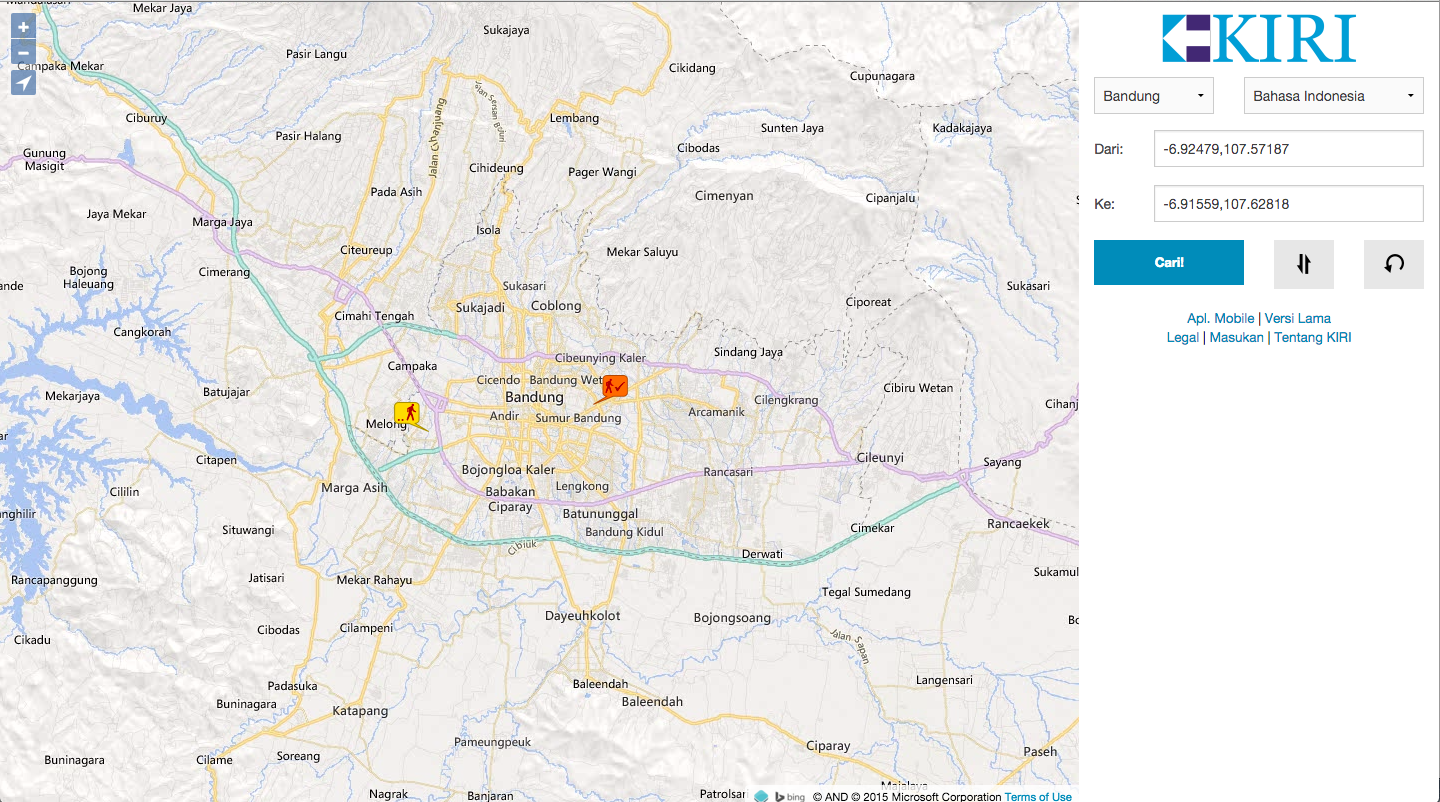
\includegraphics[scale=0.3]{Gambar/KIRI-textfield-koord}
	\caption{Input User(Klik pada peta)} 
	\label{fig:3_KIRI_textfield_koord}
\end{figure}
	
	Agar peta dapat diklik, maka memanggil method \verb!on! dengan parameter `click' dan fungsi yang akan diimplementasikan ketika melakukan klik pada peta. Isi fungsi tersebut adalah pertama melakukan pengecekan apabila textfield tempat asal atau tempat tujuan kosong, maka membuat objek \verb!ol.geom.Point! dengan parameter koordinat pada peta yang diklik oleh pengguna, lalu membuat \textit{marker} dengan gambar start.png bila textfield tempat asal kosong atau finish.png bila textfield tempat tujuan kosong. Setelah itu, menambahkan fitur marker ke \verb!inputVectorSource! yang akan ditampilkan pada peta dan menulis koordinat pada textfield tempat asal atau tempat tujuan. Kode dapat dilihat pada kode listing \ref{lst_3_php_textfield_koord_kode}.
	
	\begin{lstlisting}[caption=Membuat \textit{event} klik pada peta,label = {lst_3_php_textfield_koord_kode}]
..
// Map click event
map.on('click', function(event) {
    	if ($('#startInput').val() === '') {
		markers['start'] = new ol.Feature({
			geometry: new ol.geom.Point(event.coordinate)
		})
		markers['start'].setStyle(new ol.style.Style({
			image: new ol.style.Icon({
				src: 'images/start.png',
				anchor: [1.0, 1.0]
			})
		}));
		inputVectorSource.addFeature(markers['start']);
    		$('#startInput').val(latLngToString(ol.proj.transform(event.coordinate, 'EPSG:3857', 'EPSG:4326')));
    	} else if ($('#finishInput').val() === '') {
		markers['finish'] = new ol.Feature({
			geometry: new ol.geom.Point(event.coordinate)
		})
		markers['finish'].setStyle(new ol.style.Style({
			image: new ol.style.Icon({
				src: 'images/finish.png',
				anchor: [0.0, 1.0]
			})
		}));
		inputVectorSource.addFeature(markers['finish']);
    		$('#finishInput').val(latLngToString(ol.proj.transform(event.coordinate, 'EPSG:3857', 'EPSG:4326')));
    	}
});
..
\end{lstlisting}

\end{enumerate}

\subsubsection{Tombol Swap}
Pengguna dapat menukar isi dari \textit{textfield} tempat asal dan tujuan. Pertama kali yang dilakukan adalah mencari pada dokumen dengan \textit{id} `swapbutton' dan memanggil \textit{method} \textbf{click} dengan mengisi fungsi \textbf{swapInput} seperti pada kode listing \ref{lst_3_php_swap}. Fungsi \textbf{swapInput} berisi melakukan pencarian pada dokumen dengan \verb!id! sama dengan \verb!`startInput'! dan \verb!`finishInput'!. Melakukan penampungan sementara dengan mengambil isi dari \textit{textfield} tempat asal, lalu menukar isi dari \textit{textfield} tempat asal dan tujuan. Setelah itu, jika kedua textfield ada isinya, melakukan pencarian rute. Kode dapat diliihat pada kode listing \ref{lst_3_php_swap_fungsi}.

\begin{lstlisting}[caption=\textit{Method} untuk memanggil fungsi JavaScript ketika tombol \textit{swap} ditekan ,label = {lst_3_php_swap}]
..
$('#swapbutton').click(swapInput);
..
\end{lstlisting}

\begin{lstlisting}[caption=Fungsi JavaScript untuk menukar isi \textit{textfield} tempat asal dan tujuan ,label = {lst_3_php_swap_fungsi}]	
/**
 * Swap the inputs
 */
function swapInput() {
	var startInput = $('#startInput');
	var finishInput = $('#finishInput');
	var temp = startInput.val();
	startInput.val(finishInput.val());
	finishInput.val(temp);
	coordinates['start'] = null;
	coordinates['finish'] = null;
	if (startInput.val() != '' && finishInput.val() != '') {
		findRouteClicked();
	}
}
\end{lstlisting}

\subsubsection{Tombol Reset}
Pengguna dapat melakukan pemilihan tempat dari awal dan mengulang tampilan peta. Pertama kali yang dilakukan adalah mencari pada dokumen dengan \textit{id} `resetbutton' dan memanggil \textit{method} \verb!click! dengan mengisi fungsi \verb!resetScreen! seperti pada kode listing \ref{lst_3_php_reset}. 

\begin{lstlisting}[caption=\textit{Method} untuk memanggil fungsi JavaScript ketika tombol \textit{reset} ditekan ,label = {lst_3_php_reset}]
..
$('#resetbutton').click(resetScreen);
..
\end{lstlisting}

Fungsi resetScreen berisi berbagai fungsi seperti pada kode listing \ref{lst_3_php_reset_fungsi}, yaitu:

\begin{lstlisting}[caption=Fungsi JavaScript resetScreen ,label = {lst_3_php_reset_fungsi}]	
function resetScreen() {
	clearRoutingResultsOnTable();
	clearRoutingResultsOnMap();
	clearAlerts();
	clearStartFinishMarker();
	$.each(['start', 'finish'], function(sfIndex, sfValue) {
		var placeInput = $('#' + sfValue + 'Input');
		placeInput.val('');	
		placeInput.prop('disabled', false);
		$('#' + sfValue + 'Select').addClass('hidden');
	});
}
\end{lstlisting}

\begin{enumerate}
	\item \textbf{Fungsi clearRoutingResultsOnMap}\\
	Fungsi untuk menghapus hasil pencarian rute pada peta dan memperbarui peta sesuai dengan \verb!region! yang dipilih. Kode dapat dilihat pada kode listing \ref{lst_3_php_reset_clearMap}.
	\begin{lstlisting}[caption=Fungsi JavaScript untuk menghapus hasil pencarian rute pada peta ,label = {lst_3_php_reset_clearMap}]
	function clearRoutingResultsOnMap() {
		resultVectorSource.clear();
		updateRegion(region, false);
	}
	\end{lstlisting}
	
	\item \textbf{Fungsi clearRoutingResultsOnTable}\\
	Fungsi untuk menghapus tampilan tabel sebagai hasil pencarian rute yang akan ditampilkan pada pengguna. Kode dapat dilihat pada kode listing \ref{lst_3_php_reset_clearTable}.
	
	\begin{lstlisting}[caption=Fungsi JavaScript untuk menghapus tampilan tabel,label = {lst_3_php_reset_clearTable}]
	function clearRoutingResultsOnTable() {
		$('.tabs').remove();
		$('.tabs-content').remove();
	}
	\end{lstlisting}
	
	\item \textbf{Fungsi clearAlerts}\\
	Fungsi untuk menghapus \textit{alerts} sebagai tanda yang akan ditampilkan kepada pengguna, seperti sedang melakukan pencarian rute atau masalah koneksi. Kode dapat dilihat pada kode listing \ref{lst_3_php_reset_clearAlerts}.
	
	\begin{lstlisting}[caption=Fungsi JavaScript untuk menghilangkan \textit{alerts},label = {lst_3_php_reset_clearAlerts}]
	function clearAlerts() {
		$('.alert-box').remove();
	}
	\end{lstlisting}
	
	\item \textbf{Fungsi clearStartFinishMarker}\\
	Fungsi untuk menghapus \textit{marker} tempat awal dan tujuan, lalu menghapus fitur pada \verb!inputVectorSource!. Kode dapat dilihat pada kode listing \ref{lst_3_php_reset_clearMarker}.
	
	\begin{lstlisting}[caption=Fungsi JavaScript untuk menghilangkan \textit{alerts},label = {lst_3_php_reset_clearMarker}]
	function clearStartFinishMarker() {
		if (markers['start'] != null) {
			markers['start'] = null;
		}
		if (markers['finish'] != null) {
			markers['finish'] = null;
		}
		inputVectorSource.clear();
	}
	\end{lstlisting}
	
\end{enumerate}

\subsubsection{Tombol Find}
Pengguna dapat mencari rute untuk sampai ke tujuan (Gambar \ref{fig:3_KIRI_find}). Pengguna dapat memilih rute alternatif yang sudah disediakan KIRI jika ada (Gambar \ref{fig:3_KIRI_find_alternate}).

\begin{figure}[H]
	\centering
	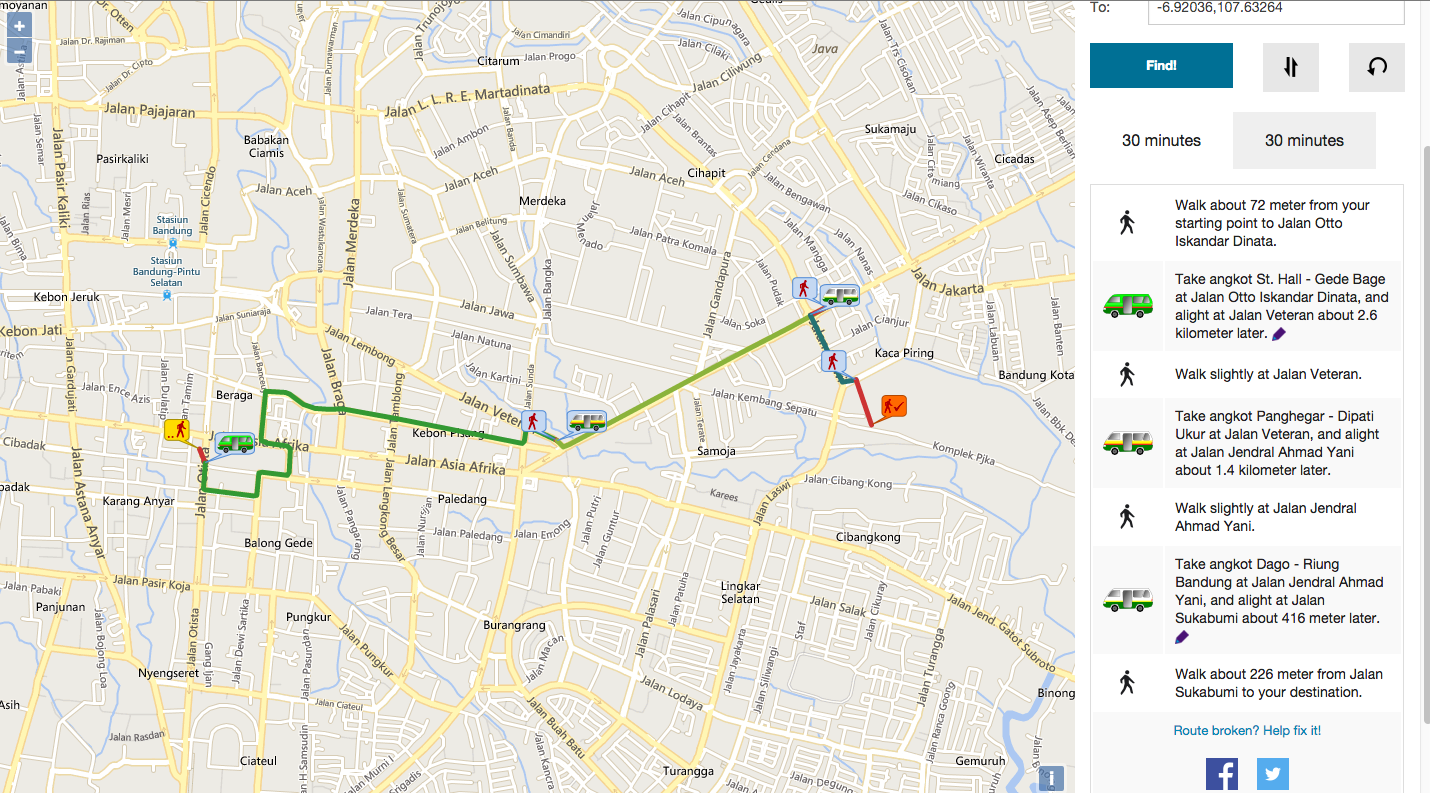
\includegraphics[scale=0.3]{Gambar/KIRI-find}
	\caption{Contoh Pencarian Rute pada KIRI} 
	\label{fig:3_KIRI_find}
\end{figure}

\begin{figure}[H]
	\centering
	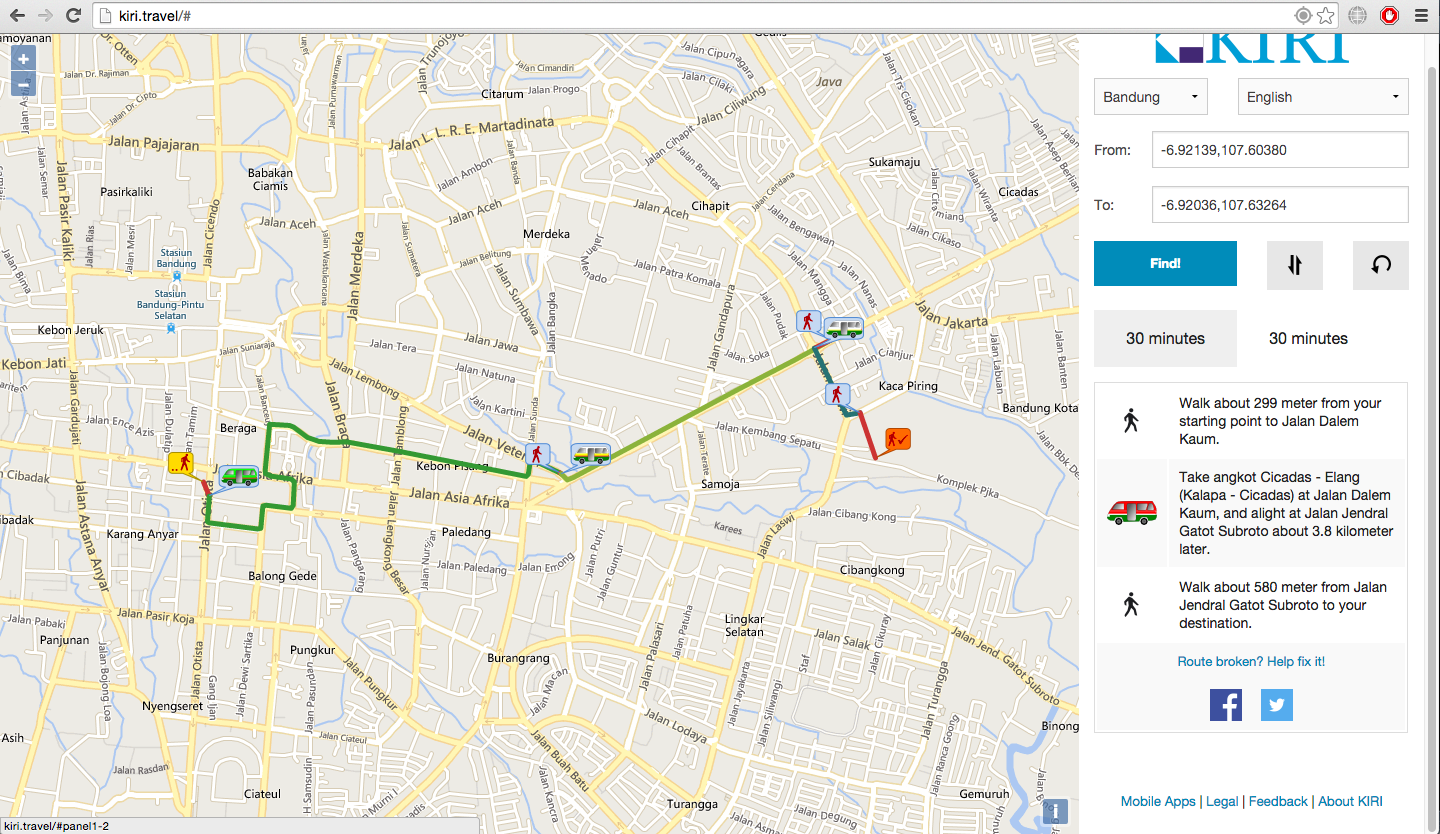
\includegraphics[scale=0.3]{Gambar/KIRI-find-alternate}
	\caption{Contoh Rute Alternatif pada KIRI} 
	\label{fig:3_KIRI_find_alternate}
\end{figure}

Hal yang pertama kali dilakukan adalah melakukan validasi jika salah satu \textit{textfield} kosong, maka akan langsung membatalkan proses dan memberi peringatan kepada pengguna. Jika tidak kosong, maka akan memunculkan peringatan `mohon menunggu' karena sedang dilakukan pencarian rute. Setelah itu melakukan pengecekan apakah isi dari \textit{textfield} merupakan format yang benar untuk garis lintang dan bujur. Jika formatnya benar, maka dimasukkan ke dalam \textit{array} \verb!coordinates! dan melakukan penambahan jumlah  completedLatLon yang berfungsi untuk mengetahui apakah kedua \textit{textfield} sudah benar formatnya untuk dilakukan pencarian rute. Jika formatnya tidak benar, maka melakukan pengecekan \textit{array} \verb!coordinates! kosong atau tidak. 
Jika kosong, maka melakukan pencarian pilihan tempat yang akan menjadi tempat sugesti yang diberikan kepada pengguna. Jika tidak kosong, maka memanggil fungsi \verb!checkCoordinatesThenRoute! dengan parameter berupa coordinates. Terakhir, melakukan pengecekan \verb!completedLatLon! jika isinya sama dengan dua, maka memanggil fungsi \verb!checkCoordinatesThenRoute!. Kode dapat dilihat pada kode listing \ref{lst_3_php_find_fungsi}.

\begin{lstlisting}[caption=Fungsi JavaScript untuk ketika tombol \textit{find} ditekan,label = {lst_3_php_find_fungsi}]
/**
 * A function that will be called when find route button is clicked
 * (or triggered by another means)
 */
function findRouteClicked() {
	// Validate
	var cancel = false;
	$.each(['start', 'finish'], function(sfIndex, sfValue) {
		if ($('#' + sfValue + 'Input').val() === '') {
			cancel = true;		
			return;
		}
	});
	if (cancel) {
		showAlert(messageFillBoth, 'alert');			
		return;
	}
	
	clearAlerts();
	clearRoutingResultsOnTable();
	showAlert(messagePleaseWait, 'secondary');
	
	var completedLatLon = 0;
	$.each(['start', 'finish'], function(sfIndex, sfValue) {
		var placeInput = $('#' + sfValue + 'Input');
		var placeSelect = $('#' + sfValue + 'Select');
		if (isLatLng(placeInput.val())) {
			coordinates[sfValue] = placeInput.val();
			completedLatLon++;
		} else {
			if (coordinates[sfValue] == null) {
				// Coordinates not yet ready, we do a search place
				protocol.searchPlace(
						placeInput.val(),
						region,
						function(result) {
							placeSelect.empty();
							placeSelect.addClass('hidden');
							if (result.status != 'error') {
								if (result.searchresult.length > 0) {
									$.each(result.searchresult, function(index, value) {
										var placeSelect = $('#' + sfValue + 'Select');
										placeSelect
									         .append($('<option></option>')
									         .attr('value',value['location'])
									         .text(value['placename']));
										placeSelect.removeClass('hidden');
									});
									coordinates[sfValue] = result.searchresult[0]['location'];
									checkCoordinatesThenRoute(coordinates);
								} else {
									clearSecondaryAlerts();
									clearRoutingResultsOnMap();
									showAlert(placeInput.val() + messageNotFound, 'alert');
								}
							} else {
								clearSecondaryAlerts();
								clearRoutingResultsOnMap();
								showAlert(messageConnectionError, 'alert');
							}
						});
			} else {
				// Coordinates are already available, skip searching
				checkCoordinatesThenRoute(coordinates);
			}
		}
	});
	if (completedLatLon == 2) {
		checkCoordinatesThenRoute(coordinates);
	}
}
\end{lstlisting}

Fungsi \textbf{checkCoordinatesThenRoute} melakukan pengecekan jika \textit{array} \verb!coordinates! tempat awal dan tempat tujuan tidak kosong maka melakukan \verb!protocol.findRoute!. \verb!protocol.findRoute! akan melakukan pencarian rute dengan koordinat tempat awal dan tujuan. Kode dapat dilihat pada kode listing \ref{lst_3_php_find_checkRoute}.
\begin{lstlisting}[caption=Fungsi JavaScript checkCoordinatesThenRoute,label = {lst_3_php_find_checkRoute}]
/**
 * Check if coordinates are complete. If yes, then start routing.
 * @param coordinates the coordinates to check.
 */
function checkCoordinatesThenRoute(coordinates) {
	if (coordinates['start'] != null && coordinates['finish'] != null) {
		protocol.findRoute(
				coordinates['start'],
				coordinates['finish'],
				locale,
				function(results) {
					if (results.status === 'ok') {
						showRoutingResults(results);
					} else {
						clearSecondaryAlerts();
						showAlert(messageConnectionError, 'alert');
					}
				});
	}
}
\end{lstlisting}

\subsection{Internationalization}
Penggunaan Internationalization (i18n) pada PHP dilakukan dengan cara deklarasi semua variabel yang akan digunakan pada proses i18n terlebih dahulu, misalnya buat file dengan nama tirtayasa\_en.php untuk Bahasa Inggris dan tirtayasa\_id.php untuk Bahasa Indonesia. Pada setiap file tersebut, masukkan \textit{script} PHP untuk menentukan teks yang keluar pada halaman \textit{web} seperti pada kode listing \ref{lst_3_i18n_en} dan kode listing \ref{lst_3_i18n_id}. 

\begin{lstlisting}[caption=Script PHP untuk Bahasa Inggris,label = {lst_3_i18n_en}]
<?php

	$index_about_kiri = "About KIRI";
	$index_apps = "Mobile Apps";
	$index_advanced_ = "Advanced...";
	$index_buyticket = "BUY TICKET";
	$index_connectionerror = 'Connection problem';
?>
\end{lstlisting}


\begin{lstlisting}[caption=Script PHP untuk Bahasa Indonesia,label = {lst_3_i18n_id}]
<?php
	$index_about_kiri = "Tentang KIRI";
	$index_apps = "Apl. Mobile";
	$index_advanced_ = "Lanjut...";
	$index_buyticket = "BUY TICKET";
	$index_connectionerror = 'Gangguan koneksi';
?>
\end{lstlisting}

Setelah itu, memuat file i18n dan masukkan \textit{script} PHP pada \textit{tag} HTML yang ingin diubah saat dilakukan i18n. Adanya \textit{script} PHP pada tag HTML, maka teks akan berubah jika dilakukan i18n seperti pada kode listing \ref{lst_3_i18n_php}.

\begin{lstlisting}[caption=Script PHP untuk Internationalization,label = {lst_3_i18n_php}]
	...
	<label for="startInput" class="inline"><?php print $index_from; ?></label>
	<label for="finishInput" class="inline"><?php print $index_to; ?></label>
	<a href="#" class="small button expand" id="findbutton"><strong><?php print $index_find; ?></strong></a>
	...
\end{lstlisting}

Untuk menentukan file mana yang akan digunakan dalam proses i18n, jangan lupa untuk memuat file yang diinginkan seperti pada kode listing \ref{lst_3_i18n_load}.
\begin{lstlisting}[caption=Script PHP untuk memuat file i18n,label = {lst_3_i18n_load}]
	...
	require_once("../etc/locale/tirtayasa_$locale.php");
	...
\end{lstlisting}

\subsection{Pencarian Rute}
Pencarian rute pada KIRI dilakukan di bagian server, yaitu pada file handle.php. Langkah awal pada handle.php dapat dijelaskan sebagai berikut:
\begin{enumerate}
	\item Memuat \textit{file} constants.php untuk menyiapkan data yang akan dipakai pada halaman web.
	\item Memuat utils.php untuk fungsi manipulasi data, koneksi basisdata, mengirimkan pencatatan, dan melakukan validasi.
	\begin{itemize}
		\item Fungsi \verb!init_mysql! untuk memuat koneksi basisdata dengan memasukkan \textit{host, username, password}, dan basisdata yang digunakan pada MySQL.
		\item Fungsi \verb!log_statistic! untuk pencatatan data pada basisdata dengan tabel \verb!`statistic'!.
		\item Fungsi \verb!die_nice! untuk mengirimkan pesan kesalahan.
		\item Fungsi \verb!check_apikey_validity! untuk pengecekan apikey yang digunakan ada atau tidak.
		\item Fungsi \verb!retrieve_from_post! untuk mengambil data pada URL dengan memanggil method \verb!$_POST! pada \textit{query} parameter URL.
		\item Fungsi \verb!retrieve_from_get! untuk mengambil data pada URL dengan memanggil method \verb!$_GET! pada \textit{query} parameter URL.
		\item Fungsi \verb!retrieve_from_cache! untuk mengambil data pada basisdata dengan tabel \verb!`cache'! dengan parameter `type' dan `cacheKey'.
		\item Fungsi \verb!put_to_cache! untuk memasukkan data pada basisdata dengan tabel \verb!`cache'! dengan parameter `type' , `cacheKey', dan `cacheValue'.
	\end{itemize}
	\item \verb!start_working! untuk menyiapkan header pada PHP.
	\begin{itemize}
		\item Fungsi \verb!header('Content-Type: application/json')! untuk menghasilkan keluaran berupa JSON.
		\item Fungsi \verb!header('Cache-control: no-cache')! digunakan pada HTTP/1.1 dan fungsi \verb!header('Pragma: no-cache')! digunakan pada HTTP/1.0. Keduanya berfungsi untuk mencegah pengguna menyimpan \textit{cache response}.
	\end{itemize}
	\item \verb!init_mysql! untuk menyiapkan koneksi basisdata.
	\item Mendapatkan data \verb!mode!, \verb!version!, dan \verb!apikey! dari \textit{method} \verb!POST! masing-masing dengan parameter `mode', `version', dan `apikey'.
	\item Jika data \verb!version! sama dengan  \verb!null!, maka isi data \verb!version! dengan 1. 
	\item Melakukan pengecekan \verb!apikey! apakah ada di basisdata atau tidak. Jika ada, cek lagi apakah ada pengecualian IP komputer pada basisdata.
\end{enumerate}

\subsubsection{Mode Findroute}
Bagian ini terletak pada baris 14-181 dari handle.php (kode \ref{lst:handle.php}). Langkah pertama yang dilakukan adalah memasukkan data \verb!start!, \verb!finish!, dan \verb!locale! dengan mendapatkan nilai \textit{method} \verb!POST! dengan parameter `start', `finish', dan `locale'. Sebelum dimasukkan, memanggil \textit{method} \verb!addslashes! yang berfungsi jika ada karakter spesial seperti ' atau " tidak dianggap sebagai suatu String yang berbeda. Setelah itu melakukan pengecekan untuk lokalisasi. Jika ada lokalisasi, memuat \textit{file} (lokalisasi Bahasa Inggris atau lokalisasi Bahasa Indonesia). Setelah itu melakukan pengecekan variabel \verb!presentation!, ada dua yaitu \verb!`mobile'! atau \verb!`desktop'!. Melakukan pengecekan version yang digunakan:
\begin{itemize}
	\item Jika \verb!version! lebih besar sama dengan 2, maka memasukkan data \verb!count! dengan 1. Jika \verb!presentation! sama dengan \verb!`mobile'!, maka memasukkan data \verb!count! dengan jumlah \textit{array} \verb!alternatives!. Setelah itu melakukan pengulangan sebanyak \verb!count! yang berisi:\\
		Menambahkan \textit{query} parameter URL \url{http://newmenjangan.cloudapp.net:8000} dengan:
		\begin{itemize}
			\item 	``?start=x'' dan ``finish=y'', dimana x adalah koordinat tempat asal dan y adalah koordinat tempat tujuan.
			\item \verb!mw!, \verb!wm!, dan \verb!pt! masing-masing dengan nilai dari \textit{array} \verb!alternative! satu persatu dengan indeks `mw', `wm', dan `pt'.
			\item memanggil fungsi \verb!file_get_content! yang akan mengembalikan \verb!FALSE! jika gagal dan mengembalikan JSON pesan kesalahan. Jika berhasil akan mendapatkan String dengan \textit{URL} \url{http://newmenjangan.cloudapp.net:8000}, pembacaan maksimal sebanyak 51200 \textit{bytes}.
			\item memasukkan ke \textit{array} \verb!results! yang mempunyai indeks `result' dengan nilai \verb!true!.
		\end{itemize}
	\item Jika \verb!version! kurang dari 2, langsung akses \textit{URL} \url{http://newmenjangan.cloudapp.net:8000} dengan \textit{query} parameter ``?start=x'' dan ``finish=y'', dimana x adalah koordinat tempat asal dan y adalah koordinat tempat tujuan.
\end{itemize}

Langkah selanjutnya adalah pengulangan sejumlah data \verb!results! menjadi \verb!result! dengan nilai yang dimasukkan ke data \verb!dummy! yang berisi:
\begin{itemize}
	\item Membuat data \verb!steps! yang berisi data \verb!result! yang telah dipisahkan per baris.
	\item Melakukan pengulangan setiap data \verb!steps! dan dimasukkan ke \verb!step! yang berisi:
	\begin{itemize}
		\item Membuang spasi yang ada pada data \verb!step!.
		\item Jika \verb!step! sama dengan \verb!`none'!, melakukan pengecekan pada banyaknya data \verb!results!. Jika banyak data \verb!results! bukan satu berarti ada rute alternatif dan akan melanjutkan ke langkah selanjutnya. Tetapi jika banyak data \verb!results! adalah satu, maka tidak ada rute alternatif.
		\item Mendaftarkan data \verb!means!, \verb!means_detail!, \verb!route!, \verb!distance!, dan \verb!nearbyplaceids! yang didapat dari data \verb!step! yang telah dipisahkan `/'. Jika salah satu data kosong, akan mengirimkan pesan kesalahan.
		\item Inisialisasi data \verb!points! yang didapat dari data \verb!route! yang sudah dipisahkan spasi, inisialisasi data \verb!from! dari data \verb!points! dengan indeks 0 dan inisialisasi data \verb!to'! dari data \verb!points! dengan indeks terakhir.
		\item Jika nilai data \verb!points! ada yang sama dengan \verb!`start'!, maka mengganti data \verb!points! tersebut dengan data \verb!start!. Jika nilai data \verb!points! ada yang sama dengan \verb!`finish'!, maka mengganti data \verb!points! tersebut dengan data \verb!finish!.
		 \item Memasukkan data \verb!humanized_from! dengan memanggil fungsi \verb!humanize_point! dengan parameter \verb!from! dan \verb!humanized_to! dengan memanggil fungsi \verb!humanize_point! dengan parameter \verb!to!.
		 \item Jika \verb!means! sama dengan \verb!`walk'!, melakukan pengecekan apakah  \verb!humanized_from! sama dengan \verb!humanized_to!. Jika \verb!presentation! tidak sama dengan \verb!mobile!, maka memasukkan \verb!message_walk_samestreet! ke variabel \verb!humanreadable!. Mengganti \verb!from! yang ada di \verb!humanreadable! dengan nilai \verb!humanized_from!, mengganti \verb!distance! yang ada di \verb!humanreadable! dengan nilai \verb!distance! yang dipresentasikan sesuai format wilayah pengguna. Lalu menghitung waktu tempuh yang dibutuhkan.
		 \item Jika \verb!means! tidak sama dengan \verb!`walk'!, melakukan pencarian pada tabel \verb!tracks! digabung dengan \verb!tracktypes! dengan kolom nama jalur, tipe jalur yang digunakan, \textit{URL} untuk melakukan pemesanan (jika XTrans), kecepatan transportasi, dan informasi internal jalur dengan syarat:
				\begin{enumerate}
					\item \verb!trackTypeId! sama dengan \verb!means! pada tabel \verb!tracktypes! dan \verb!tracks!.
					\item \verb!trackid! sama dengan \verb!means_detail! pada tabel \verb!tracks!.
				\end{enumerate}						 
		  Jika ada hasil dari pencarian, maka: 
		  \begin{enumerate}
		  		\item Memasukkan nilai \verb!trackname! dari tabel \verb!tracks! ke \verb!readable_track_name!.
		  		\item Memasukkan nilai \verb!nama! dari tabel \verb!tracktypes! ke \verb!track_type_name!.
		  		\item Memasukkan nilai \verb!speed! dari tabel \verb!tracktypes! ke data \verb!speed! yang sudah dijadikan format angka.
		  \end{enumerate}
		  Lalu melanjutkan pengecekan apakah \verb!presentation! sama dengan \verb!`mobile'!. Jika \verb!presentation! sama dengan \verb!`mobile'!, maka menambahkan data \verb!humanized_from! dengan \verb!`%fromicon'! dan \verb!humanized_to! dengan \verb!`%toicon'!. Setelah itu, memasukkan \verb!message_angkot! ke data \verb!humanreadable!. Memperbarui nilai \verb!humanreadable! dengan mengganti:
		  
		  \begin{itemize}
		  		\item \verb!%from! dengan nilai dari \verb!humanized_from!.
		  		\item \verb!%to! dengan nilai dari \verb!humanized_to!.
		  		\item \verb!%distance! dengan nilai dari \verb!distance! yang dipresentasikan sesuai format wilayah pengguna.
		  		\item \verb!%trackname! dengan nilai dari \verb!readable_track_name!.
		  		\item \verb!%tracktype! dengan nilai dari \verb!track_type_name!.		  		
		  \end{itemize}
		 Setelah itu, menghitung waktu tempuh dari data \verb!distance! dibagi dengan data \verb!speed!. Melakukan pengecekan nilai \verb!URL! dari tabel \verb!tracktypes! dan nilai  \verb!extraParameters! dari tabel \verb!tracktypes! kosong tidak. Jika tidak kosong maka menambahkan data \verb!booking_url! dengan menambahkan nilai \verb!URL! dari tabel \verb!tracktypes! dan nilai  \verb!extraParameters! dari tabel \verb!tracktypes!. 
		 Lalu melakukan pengecekan nilai \verb!internalinfo! dari tabel \verb!tracks! dimulai dengan \verb!`angkotwebid:'!. Jika dimulai dengan \verb!`angkotwebid:'!, maka mendapatkan \textit{array} \verb!token! dengan memisahkan `:' pada \verb!internalInfo!. Memasukkan data  \verb!editor_url! yang berisi awalan \textit{URL} angkotwebid, \verb!token! dengan indeks kedua, dan akhiran \textit{URL} angkotwebid. 
		 \item Jika \verb!humanreadable! tidak sama dengan \verb!null!, maka memasukkan \verb!route_output! dengan isi \textit{array} dari \verb!means!, \verb!means_detail!, \verb!points!,  \verb!humanreadable!, \verb!booking_url!, dan \verb!editor_url!. 
	\end{itemize}
	\item Memasukkan \verb!routing_result! dengan indeks \verb!steps! dengan nilai dari  \verb!route_output!.
	\item Memasukkan \verb!routing_result! dengan indeks \verb!traveltime! dengan nilai jam dan menit dari \verb!travel_time! yang sudah dilakukan i18n.
	\item Memasukkan data \verb!routing_result! ke dalam \textit{array} \verb!routing_results!.
\end{itemize}
Setelah itu, memasukkan data ke tabel statistik dengan parameter:
	\begin{itemize}
		\item \verb!apikey! yang digunakan.
		\item \verb!FINDROUTE! merupakan tipe statistik yang dimasukkan.
		\item \verb!$start/$finish/sizeof($results)! merupakan keterangan statistik dimana \verb!$start! adalah titik koordinat tempat asal, \verb!$finish! adalah titik koordinat tempat tujuan, dan \verb!sizeof($results)! adalah jumlah dari data \verb!$results!.
	\end{itemize}
Lalu menutup koneksi ke basisdata. Jika \verb!version! tidak sama dengan \verb!null! dan \verb!version! lebih besar sama dengan 2, maka print hasil yang sudah di \textit{encode} menjadi JSON, yaitu:
	\begin{itemize}
		\item \verb!status! dengan nilai \verb!`ok'!
		\item \verb!routingresults! dengan nilai \verb!routing_results! yang merupakan hasil pencarian rute.
	\end{itemize}
Jika \verb!version! sama dengan \verb!null! dan \verb!version! kurang dari 2, maka print hasil yang sudah di \textit{encode} menjadi JSON, yaitu:
	\begin{itemize}
		\item \verb!status! dengan nilai \verb!`ok'!
		\item \verb!routingresult! dengan nilai \verb!routing_results! dengan indeks ke nol dan memiliki \textit{key} berupa \verb!steps! yang merupakan hasil pencarian rute.
		\item \verb!traveltime! dengan nilai \verb!routing_results! dengan indeks ke nol dan memiliki \textit{key} berupa \verb!traveltime! yang merupakan waktu tempuh.
	\end{itemize}

\subsubsection{Mode Search}
Bagian ini terletak pada baris 183-280 dari handle.php (kode \ref{lst:handle.php}). Langkah pertama yang dilakukan adalah memasukkan data \verb!querystring!, \verb!apikey!, dan \verb!region! dengan mendapatkan nilai \textit{method} \verb!POST! masing-masing dengan parameter `querystring', `apikey', dan `region'. Jika \verb!region! sama dengan \verb!null!, maka isi \verb!region! dengan \verb!`bandung!. Melakukan pengulangan sejumlah data \verb!regioninfos! dengan nilai yang dimasukkan ke data \verb!value! yang berisi:
\begin{itemize}
	\item Mencari dalam \verb!querystring! ada \textit{pattern} \verb!`/searchplace'! dimana \verb!`searchplace'! diambil dari \verb!value! dengan \textit{key} \verb!`searchplace_regex'! dan tampilkan pada \textit{array} \verb!matches!. Jika terdapat \textit{pattern} tersebut, maka memasukkan data \verb!region! dengan nilai \verb!key!, memperbarui \verb!querystring! dengan mengambil panjang kalimat dari indeks nol sampai dengan indeks ditemukannya \textit{pattern} tersebut.
	\item Mengubah \verb!querystring! menjadi format \textit{URL}.
	\item Memasukkan data \verb!cached_searchplace! dengan mengambil data dari tabel \verb!cache! dengan tipe \verb!searchplace! dan \textit{key} \verb!region/querystring!. Jika \verb!cached_searchplace! tidak sama dengan \verb!null!, maka membuat JSON untuk \textit{output} dengan:
	\begin{itemize}
		\item \verb!status! dengan nilai \verb!`ok'!
		\item \verb!searchresult! dengan nilai \verb!cached_searchplace!
		\item \verb!attributions! dengan nilai \verb!null!
	\end{itemize}
	Jika \verb!cached_searchplace! sama dengan \verb!null!, memasukkan data \verb!lat!, \verb!lon!, dan \verb!radius! yang diambil dari \verb!regioninfos! dengan indeks \verb!`region'! dan \textit{key} \verb!`lat'!, \verb!`lon'!, dan \verb!`radius'!. Memasukkan \verb!result! dengan hasil akses \textit{URL} dari data \verb!`full_url'!. Jika \verb!result! sama dengan \verb!FALSE! atau jumlah \verb!result! lebih besar dari \verb!maximum_http_response_size!, maka mengeluarkan pesan kesalahan. 
	Setelah itu, memasukkan \verb!json_result! dengan mengubah format JSON menjadi String dari data \verb!result!. Jika \verb!json_result! dengan indeks \verb!`status'! adalah \verb!`OK'! atau \verb!`ZERO_RESULTS'!, maka menyiapkan \textit{array} \verb!search_result!. Jika hasilnya \verb!`ZERO_RESULTS'!, maka mengeluarkan catatan kesalahan dan memperbarui data \verb!size! menjadi 0. Jika hasilnya \verb!`OK'!, maka mengambil angka minimal antara banyaknya data \verb!json_result! dengan indeks \verb!`results'! dan \verb!search_maxresult!. Melakukan pengulangan dari nol sampai dengan \verb!size! yang dinisialkan dengan \verb!i!:
	\begin{itemize}
		\item Memasukkan data \verb!current_venue! dengan \verb!json_result! indeks results dengan \textit{key} \verb!i!.
		\item Memasukkan data \verb!search_result! dengan indeks \verb!i! dan \textit{key} \verb!placename! yang isinya adalah \verb!current_venue! dengan indeks \verb!name!.
		\item Memasukkan data \verb!search_result! dengan indeks \verb!i! dan key \verb!`location'! yang isinya adalah String yang sudah diformat \verb!`%.latlonlf%.latlonlf'! yang nilainya diambil dari \verb!current_venue! dengan indeks \verb!`geometry'! dan \verb!`location'! dengan \textit{key} \verb!`lat'! dan \verb!`lng'!.
		\item Menyiapkan \verb!json_output! yang merupakan \textit{array} dari:
		\begin{itemize}
			\item \verb!status! dengan nilai \verb!`ok'!
			\item \verb!searchresult! dengan nilai \verb!search_result! yang merupakan hasil pencarian rute
			\item \verb!attributions! dengan nilai \verb!null!
		\end{itemize}
		\item Mengirim catatan dengan \verb!apikey! yang digunakan.
		\item Memasukkan data ke tabel \textit{cache} dengan tipe \verb!`cache_searchplace'! dan \textit{key} \verb!region/querystring! yang berisi JSON \verb!search_result!.
	\end{itemize}
	\item Mengeluarkan hasil JSON \verb!json_output!.
\end{itemize}

\subsubsection{Mode Reporterror}
Bagian ini terletak pada baris 282-284 dari handle.php (kode \ref{lst:handle.php}). Langkah pertama yang dilakukan adalah mendapatkan \verb!errorcode! dari \textit{method} \verb!POST! dengan parameter \verb!`errorcode'!. Mencatat kesalahan dan dimasukkan ke dalam \textit{file}. Mengeluarkan JSON dengan:
\begin{itemize}
			\item \verb!status! dengan nilai \verb!`ok'!
\end{itemize} 
dan memberhentikan eksekusi program.

\subsubsection{Mode Nearbytransport}
Bagian ini terletak pada baris 286-313 dari handle.php (kode \ref{lst:handle.php}). Langkah pertama yang dilakukan adalah mendapatkan \verb!start! dari \textit{method} \verb!POST! dengan parameter \verb!`routestart'!. Jika \verb!version! lebih besar sama dengan 2, maka membuat data \verb!lines! dengan mendapatkan String dari \textit{URL} \url{http://newmenjangan.cloudapp.net:8000} dengan \textit{query} parameter ``/?start=\$start''. Setelah mendapatkan hasil, lakukan pemisahan baris. Melakukan pengulangan sebanyak \verb!lines! yang berisi:
\begin{itemize}
	\item Melakukan pemisahan \verb!`\'! dari \verb!line!, lalu mendaftarkan data menjadi  \verb!tracktypeid!, \verb!trackid!,dan \verb!distance!.
	\item Membuat data \verb!result! dengan eksekusi \textit{statement} SQL, yaitu mendapatkan \verb!trackname! dari tabel \verb!tracks! dimana kolom \verb!trackid! dan \verb!tracktypeid! sesuai dengan data \verb!tracktypeid! dan \verb!trackid!.
	\item Membuat data \verb!row! dengan mengambil hasil data \verb!result! dan melakukan pengulangan yang berisi:
	\begin{itemize}
		\item Membuat data \verb!trackName! dengan mengambil \verb!row! dengan indeks nol.
		\item Membuat data \verb!nearby_result! yang merupakan \textit{array} dari \verb!trackTypeId'!, \verb!trackId!, \verb!trackName!, dan \verb!distance!.
	\end{itemize}
	\item Menyortir \textit{array} \verb!nearby_result! berdasarkan fungsi \verb!nearby_result_compare!. Fungsi \verb!nearby_result_compare! membandingkan jarak yang diambil dari \textit{array} dengan indeks ketiga.
	\item Memasukkan data ke tabel statistik dengan parameter:
	\begin{itemize}
		\item \verb!apikey! yang digunakan.
		\item \verb!NEARBYTRANSPORTS! merupakan tipe statistik yang dimasukkan.
		\item \verb!$start! merupakan keterangan statistik dimana \verb!$start! adalah titik koordinat tempat asal dan jumlah dari data \verb!$results!.
	\end{itemize}
	\item Mengeluarkan JSON dengan:
\begin{itemize}
			\item \verb!status! dengan nilai \verb!`ok'!
			\item \verb!nearbytransports! dengan nilai \verb!nearby_result!
\end{itemize} 
	
\end{itemize}

\subsubsection{Fungsi humanize\_point}
Tujuan dari fungsi ini adalah merubah lokasi dalam bentuk \textit{point} menjadi nama lokasi tempat dari \textit{point} tersebut. Fungsi ini menerima parameter \verb!location! yang merupakan String. Fungsi ini berisi sebagai berikut:
\begin{itemize}
	\item Melakukan deklarasi variabel \textit{global} untuk digunakan.
	\item Melakukan pengecekan data \verb!location!. Jika \verb!location! sama dengan \verb!`start'! maka mengembalikan \verb!message_start!. Jika \verb!location! sama dengan \verb!`finish'!, maka mengembalikan \verb!message_finish!.
	\item Jika bukan keduanya, maka memanggil fungsi \verb!mysqli_escape_string!.
	\item Melakukan pengecekan pada tabel \textit{cache} ada atau tidak dengan \textit{key} \verb!cache_geocoding! dan bernilai sesuai dengan parameter \verb!location! atau tidak dan dimasukkan ke data \verb!cached_geocode!. Jika ada nilainya, langsung mengembalikan nilai tersebut.
	\item Jika tidak ada, maka akan menambahkan \textit{query} parameter ``?key=\$gmaps\_server\_key\&latlng=\$location\&sensor=false'' pada \textit{URL} \url{https://maps.googleapis.com/maps/api/geocode/json} dimana \verb!gmaps_server_key! adalah \textit{key} untuk API Google dan \verb!latlng! adalah garis lintang dan garis bujur. Jika berhasil akses dan mendapatkan \verb!status! sama dengan \verb!`OK'!, maka akan menambahkan lokasi sugesti pada pengguna. Jika \verb!status! tidak sama dengan \verb!`OK'!, maka akan menampilkan pesan kesalahan. 
\end{itemize}
\section{Analisis Sistem Usulan}
\label{sec:perubahan}

\subsection{Peta}
Peta pada sistem usulan menggunakan OpenLayers yang sama dengan sistem kini.

\subsection{Form Samping}
\subsubsection{Dropdown Menu Kota}
Untuk menampilkan pilihan kota pada \play, menampilkan semua pilihan kota yang terdapat pada KIRI dan melakukan validasi \verb!location!. Kode dapat dilihat pada kode listing \ref{lst_3_play_dropdown_kota_tampilan}

\begin{lstlisting}[caption=Menampilkan pilihan kota kepada pengguna ,label = {lst_3_play_dropdown_kota_tampilan}]
..
<select class="fullwidth" id="regionselect">
    	@for(regioninfo <- regioninfos) {
         <option value=@regioninfo._1
                 @if(regioninfo._1 == region){
                          selected
                  }
          >@regioninfo._2.getName</option>
      }
</select>
..
\end{lstlisting}

\subsubsection{Dropdown Menu Bahasa}
Untuk menampilkan pilihan bahasa, menggunakan \textit{tag} HTML \verb!option!. Pada bagian ini. Kode dapat dilihat pada \ref{lst_3_play_dropdown_bahasa_tampilan}

\begin{lstlisting}[caption=Menampilkan pilihan bahasa kepada pengguna ,label = {lst_3_play_dropdown_bahasa_tampilan}]
..
<select class="fullwidth" id="localeselect">
          <option value="en">English</option>
          <option value="id"
                   @if(locale == "id"){
                            selected
                     }
        >Bahasa Indonesia</option>
</select>
..
\end{lstlisting}

\subsubsection{Textfield}
Pada \play, \textit{textfield} pada KIRI dibuat  agar dapat dilakukan proses i18n, seperti pada kode listing \ref{lst_3_play_textfield_from} untuk \textit{textfield} tempat asal dan kode listing \ref{lst_3_play_textfield_to} untuk \textit{textfield} tempat tujuan.

\begin{lstlisting}[caption=Menampilkan \textit{textfield} tempat awal kepada pengguna ,label = {lst_3_play_textfield_from}]
..
<div class="small-2 columns">
    <label for="startInput" class="inline">@Messages.get("from")</label>
</div>
<div class="small-10 columns">
    <input type="text" id="startInput" value=""
    placeholder="@Messages.get("ph_from")">
</div>
..
\end{lstlisting}

\begin{lstlisting}[caption=Menampilkan \textit{textfield} tempat tujuan kepada pengguna ,label = {lst_3_play_textfield_to}]
..
<div class="small-2 columns">
    <label for="finishInput" class="inline">@Messages.get("to")</label>
</div>
<div class="small-10 columns">
    <input type="text" id="finishInput" value=""
    placeholder="@Messages.get("ph_to")">
</div>
..
\end{lstlisting}
	
Pada \play, hal yang diubah adalah pengambilan gambar pada folder `assets/images'. Kode dapat dilihat pada kode listing \ref{lst_3_play_textfield_koord_kode}.
	
	\begin{lstlisting}[caption=Membuat \textit{event} klik pada peta,label = {lst_3_play_textfield_koord_kode}]
//for map click event
map.on('click', function(event) {
    if (startInput.value === '')
    {
        markers['start'] = new ol.Feature({
            geometry: new ol.geom.Point(event.coordinate)
        })
        markers['start'].setStyle(new ol.style.Style({
            image: new ol.style.Icon({
                src: '/assets/images/start.png',
                anchor: [1.0, 1.0]
            })
        }));
        inputVectorSource.addFeature(markers['start']);
        startInput.value = latLngToString(ol.proj.transform(event.coordinate, 'EPSG:3857', 'EPSG:4326'));
    }else if (finishInput.value === '') {
        markers['finish'] = new ol.Feature({
            geometry: new ol.geom.Point(event.coordinate)
        })
        markers['finish'].setStyle(new ol.style.Style({
            image: new ol.style.Icon({
                src: 'assets/images/finish.png',
                anchor: [0.0, 1.0]
            })
        }));
        inputVectorSource.addFeature(markers['finish']);
        finishInput.value = latLngToString(ol.proj.transform(event.coordinate, 'EPSG:3857', 'EPSG:4326'));
    }
});

\end{lstlisting}

\subsubsection{Tombol Swap}
Fungsi tombol Swap menggunakan sistem yang sudah ada karena menggunakan JavaScript.

\subsubsection{Tombol Reset}
Fungsi tombol Reset menggunakan sistem yang sudah ada karena menggunakan JavaScript.

\subsubsection{Tombol Find}
Fungsi tombol Find menggunakan sistem yang sudah ada karena menggunakan JavaScript.


\subsection{Internationalization}
Penggunaan i18n pada \play hampir sama dengan i18n pada PHP, pertama deklarasi semua variabel yang akan digunakan pada i18n, misal membuat file dengan nama messages.en untuk Bahasa Inggris dan messages.id untuk Bahasa Indonesia. Pada setiap file tersebut, masukkan kunci beserta value untuk untuk menentukan teks yang keluar pada halaman web seperti pada kode listing \ref{lst_3_i18n_play_en} dan kode listing \ref{lst_3_i18n_play_id}.

\begin{lstlisting}[caption=Script \play untuk Bahasa Inggris,label = {lst_3_i18n_play_en}]
from = From:
ph_from = e.g. Stasiun
ph_to = e.g. Monas,Jakarta
find = Find!
to = To:
...
\end{lstlisting}


\begin{lstlisting}[caption=Script \play untuk Bahasa Indonesia,label = {lst_3_i18n_play_id}]
from = Dari:
ph_from = misal: Stasiun
ph_to = misal: Monas, Jakarta
find = Cari!
to = Ke:
...
\end{lstlisting}

Pada \play, ada dua cara untuk melakukan i18n dan sudah tersedia metode untuk melakukan i18n, yaitu:
\begin{enumerate}
	\item Memanggil \textit{method} @Messages dengan parameter berupa String yang merupakan kunci dari file messages.LANG. Tetapi, dengan menggunakan cara ini, perlu dilakukan memuat ulang dua kali halaman \textit{web}. Kode dapat dilihat pada \ref{lst_3_i18n_play_1}
	
	\begin{lstlisting}[caption=Script \play untuk Internationalization,label = {lst_3_i18n_play_1}]
		..
		<label for="startInput" class="inline">@Messages("from")</label>
		<label for="finishInput" class="inline">@Messages("to")</label>
		<a href="#" class="small button expand" id="findbutton"><strong>@Messages("find")</strong></a>
		...
	\end{lstlisting}
	
	
	\item Melakukan @import play.i18n.\_ pada \textit{template view} dan menggunakan \textit{method} \@Messages.get dengan parameter berupa String yang merupakan kunci dari file messages.LANG. Kode dapat dilihat pada \ref{lst_3_i18n_play_2}.
	
		\begin{lstlisting}[caption=Script \play untuk Internationalization,label = {lst_3_i18n_play_2}]
		@import play.i18n._
		..
		<label for="startInput" class="inline">@Messages.get("from")</label>
		<label for="finishInput" class="inline">@Messages.get("to")</label>
		<a href="#" class="small button expand" id="findbutton"><strong>@Messages.get("find")</strong></a>
	\end{lstlisting}
	
\end{enumerate}

\subsection{Pencarian Rute}
Algoritma yang digunakan pada sistem usulan sama, tetapi ada beberapa struktur data yang berbeda yang akan dijelaskan sebagai berikut:
\begin{itemize}
	\item Menyiapkan header pada aplikasi dengan menggunakan objek \verb!response! dengan \textit{method}:
	\begin{itemize}
		\item Fungsi \verb!setContentType! untuk menghasilkan \textit{output} dengan tipe tertentu.
		\item Fungsi \verb!setHeader! untuk mengatur \textit{header} pada aplikasi.
	\end{itemize}
	\item \textit{Array} pada Java menggunakan HashMap dan arrayList karena \textit{array} mengandung indeks dan \textit{key} tertentu.
	\item Koneksi pada aplikasi menggunakan JDBC.
	\item Hasil eksekusi \textit{statement} SQL dimulai dari indeks ke satu, bukan nol.
	\item StringBuilder untuk menghasilkan output pada aplikasi.
	\item Melakukan format JSON dengan menggunakan ObjectNode.
	\item Melakukan \textit{encode} JSON menggunakan JsonNode.
	\item Melakukan perhitungan matematika dengan menggunakan kelas Math.
\end{itemize}

\section{Analisis Use Case}
\label{sec:usecase}
Diagram \textit{use case} pada KIRI hanya mempunyai satu aktor, yaitu pengguna. Diagram \textit{use case} dapat dilihat pada gambar \ref{fig:3_usecase}.

\begin{figure}[H]
	\centering
	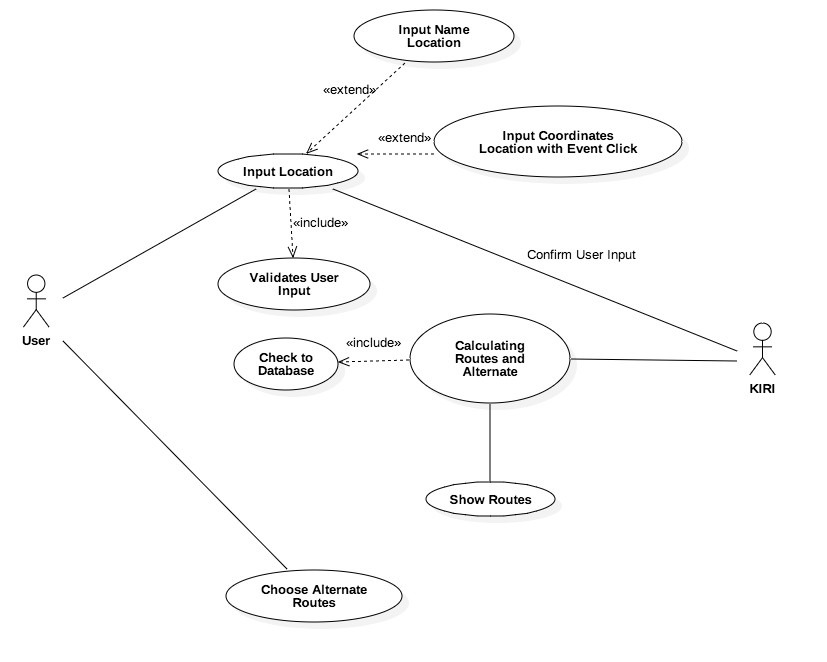
\includegraphics[scale=0.5]{Gambar/usecase}
	\caption{Use Case Diagram KIRI} 
	\label{fig:3_usecase}
\end{figure}

Terdapat empat \textit{use case}, yaitu:
\begin{enumerate}
	\item \textbf{Memasukkan lokasi}, pengguna dapat memasukkan lokasi dengan memasukkan nama lokasi ataupun melakukan klik pada peta dan diubah menjadi koordinat.
	\item \textbf{Memilih rute alternatif}, pengguna dapat memilih rute alternatif (jika ada) setelah proses pencarian rute.
	\item \textbf{Mengganti bahasa}, pengguna dapat memilih bahasa yang ingin digunakan dengan bahasa yang disediakan, Bahasa Indonesia atau Bahasa Inggris.
	\item \textbf{Mengganti lokasi kota}, pengguna dapat memilih lokasi kota mana yang ingin digunakan dengan pilihan kota yang disediakan, yaitu: Bandung, Jakarta, Surabaya, dan Malang.
	
\end{enumerate}

\subsection{Skenario Use Case}
\begin{enumerate}
	\item \textbf{Memasukkan lokasi}
	\begin{itemize}
			\item Nama: Memasukkan lokasi
			\item Aktor: Pengguna
			\item Deskripsi: Memasukkan lokasi dengan memasukkan nama lokasi ataupun melakukan klik pada peta dan diubah menjadi koordinat.
			\item Kondisi awal: -
			\item Kondisi akhir: Pencarian rute dan rute alternatif (jika ada) yang akan ditampilkan pada pengguna berupa rute pada peta dan penjelasan rute.
			\item Skenario utama: \\ \\
				\begin{tabular}{|p{0.5cm} |p{6cm}| p{6cm}|}
						\hline
							No 	& Aksi Aktor & Reaksi Sistem \\ \hline
							1 	& Pengguna memasukkan lokasi 	&	Sistem mendapatkan lokasi kemudian menampilkan hasil pencarian rute \\ \hline 
						\end{tabular} 
			\item Eksepsi: Rute tidak ditemukan.
		\end{itemize}
	\item \textbf{Memilih rute alternatif}
	\begin{itemize}
			\item Nama: Memilih rute alternatif
			\item Aktor: Pengguna
			\item Deskripsi: Memilih rute alternatif.
			\item Kondisi awal: Pencarian rute sudah berhasil dan ada rute alternatif
			\item Kondisi akhir: Menampilkan kepada pengguna rute alternatif pada peta beserta penjelasannya.
			\item Skenario utama: \\ \\
				\begin{tabular}{|p{0.5cm} |p{6cm}| p{6cm}|}
						\hline
							No 	& Aksi Aktor & Reaksi Sistem \\ \hline
							1 	& Pengguna memilih rute alternatif 	&	Sistem menampilkan pencarian rute alternatif pada peta dan penjelasannya \\ \hline 
						\end{tabular} 
			\item Eksepsi: Tidak ada rute alternatif.
		\end{itemize}
	\item \textbf{Mengganti bahasa}
	\begin{itemize}
			\item Nama: Mengganti bahasa
			\item Aktor: Pengguna
			\item Deskripsi: Memilih opsi bahasa yang akan digunakan.
			\item Kondisi awal: -
			\item Kondisi akhir: Menampilkan aplikasi dengan bahasa yang dipilih
			\item Skenario utama: \\ \\
				\begin{tabular}{|p{0.5cm} |p{6cm}| p{6cm}|}
						\hline
							No 	& Aksi Aktor & Reaksi Sistem \\ \hline
							1 	& Pengguna memilih opsi bahasa 	&	Sistem menampilkan tampilan dengan bahasa yang dipilih oleh pengguna \\ \hline 
						\end{tabular} 
			\item Eksepsi: -
		\end{itemize}
	\item \textbf{Mengganti lokasi kota}
	\begin{itemize}
			\item Nama: Mengganti lokasi kota
			\item Aktor: Pengguna
			\item Deskripsi: Memilih opsi lokasi kota yang akan ditampilkan pada peta dan pencarian rute pada kota tersebut.
			\item Kondisi awal: -
			\item Kondisi akhir: Menampilkan peta dengan lokasi kota yang dipilih
			\item Skenario utama: \\ \\
				\begin{tabular}{|p{0.5cm} |p{6cm}| p{6cm}|}
						\hline
							No 	& Aksi Aktor & Reaksi Sistem \\ \hline
							1 	& Pengguna memilih opsi lokasi kota 	&	Sistem menampilkan peta dengan lokasi kota yang dipilih dan menyiapkan pencarian rute pada kota tersebut \\ \hline 
						\end{tabular} 
			\item Eksepsi: -
		\end{itemize}
\end{enumerate}


\section{Analisis Activity Diagram}
\label{sec:activitydiagram}
Diagram aktivitas KIRI dapat dilihat pada \ref{fig:3_activitydiagram}.

\begin{figure}[H]
	\centering
	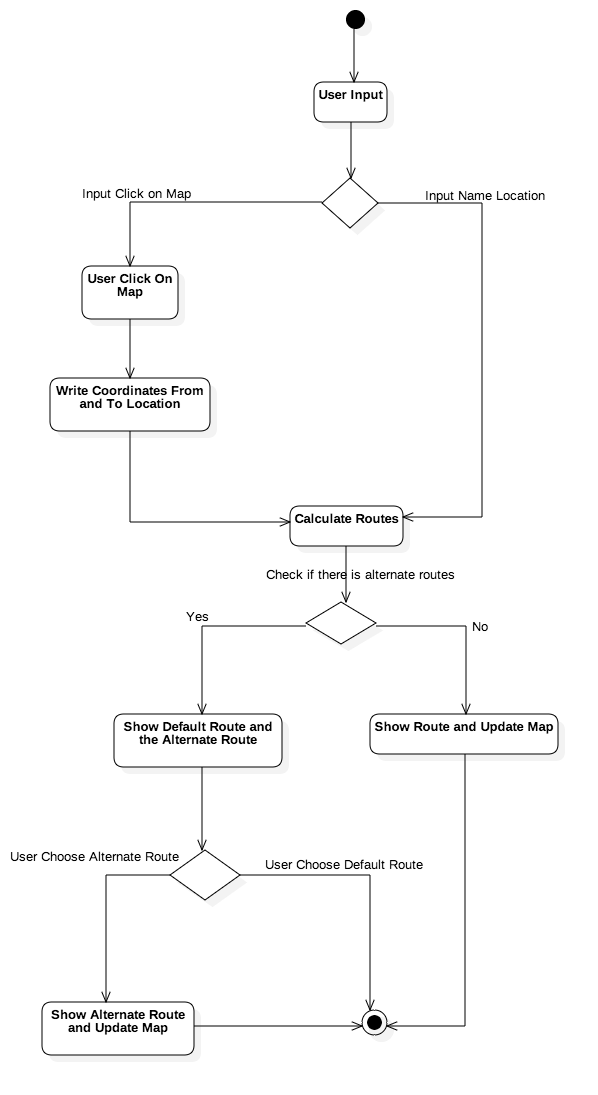
\includegraphics[scale=0.5]{Gambar/activitydiagram}
	\caption{Activity Diagram KIRI} 
	\label{fig:3_activitydiagram}
\end{figure}

Aktivitas-aktivitas yang ada pada KIRI dapat dijelaskan sebagai berikut:

\begin{enumerate}
	\item Pengguna memberikan masukan. Masukan dapat berupa dua, yaitu:
	\begin{itemize}
		\item Masukan berupa nama lokasi.
		\item Masukan berupa klik pada peta. Pengguna klik pada peta, kemudian sistem mendapatkan koordinat pada lokasi yang diklik pengguna dan menulis koordinat tersebut pada \textit{textfield} tempat asal atau tujuan.
	\end{itemize}
	\item Sistem melakukan proses pencarian rute dan melakukan pengecekan apakah ada rute alternatif atau tidak.
	\begin{itemize}
		\item Jika tidak ada rute alternatif, maka menunjukkan rute dan memperbarui peta.
		\item Jika ada rute alternatif, menunjukkan pada pengguna rute \textit{default} dan rute alternatif.
	\end{itemize}
	\item Pengguna memilih rute default atau rute alternatif.
	\begin{itemize}
		\item Jika pengguna memilih rute default, aktivitas selesai.
		\item Jika pengguna memilih rute alternatif, maka sistem menunjukkan rute alternatif dan memperbarui peta.
	\end{itemize}
\end{enumerate}


\section{Analisis Kelas}
\label{sec:kelasdiagram}
Diagram kelas analisis KIRI dapat dilihat pada \ref{fig:3_classdiagram}.

\begin{figure}[H]
	\centering
	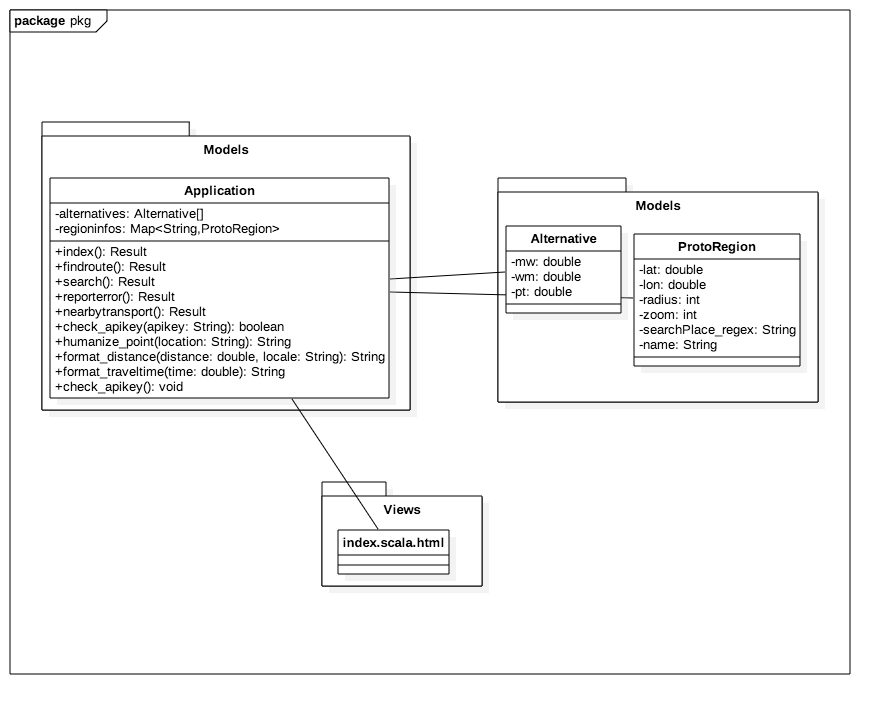
\includegraphics[scale=0.6]{Gambar/Class-Diagram-Analisis}
	\caption{Diagram Kelas Analisis KIRI} 
	\label{fig:3_classdiagram}
\end{figure}

Kelas-kelas yang ada pada KIRI dapat dijelaskan sebagai berikut:

\begin{enumerate}
	\item Application\\
			Kelas ini berfungsi untuk menghubungkan \textit{model} dengan \textit{view} dan berada pada \textit{package} controllers.
	\item Alternative\\
			Kelas untuk merepresentasikan alternatif rute yang akan dicari dan berada pada \textit{package} models.
	\item ProtoRegion\\
			Kelas untuk merepresentasikan detail kota yang disediakan KIRI dan berada pada \textit{package} models.
\end{enumerate}
